\section{Fundamentação Ponte H}
Os motores de corrente contínua trabalham nos dois sentidos de rotação quando invertidas suas polaridades. A ponte H é um circuito que tem a função de controlar esse sentido de rotação do motor a partir da inversão de sua polaridade. O exemplo a seguir, ilustra uma ponte H composta de quatro transistores que trabalham em pares nas diagonais. Basicamente, quando se aciona uma chave tem-se 12V e a outra chave-par leva o terra (0V) para o motor. A utilização de  NPN e PNP é aconselhável para evitar uma perda de tensão maior entre eles, dessa forma, a carga (motor) fica sempre ligado aos coletores dos transistores.      

\section{Fundamentação Plantário}
Na hidroponia, o cultivo das hortaliças é feito em um lugar pequeno e que não gera resíduos no local (como quando utilizado areia ou terra). De acordo com Silva et al. \cite{SILVA}, do grupo de fruticultura da Universidade Federal de Uberlândia, o pioneiro na aplicação da técnica de hidroponia foi Allen Cooper, no Glasshouse Crop Research Institute, na Inglaterra, em 1965. Cooper relatava que “a espessura do fluxo da solução nutritiva que passa através das raízes das plantas deve ser bastante pequeno (laminar), de tal maneira que as raízes não ficassem totalmente submergidas, faltando-lhes o necessário oxigênio” \cite{SILVA}. No Brasil, o método é amplamente difundido por meio de estruturas de PVC, que alocam as hortaliças e por onde flui água, que é oriunda de um reservatório e se destina ao mesmo reservatório após o caminho do plantio ser percorrido. A fim de ocupar o espaço disposto de forma otimizada, trabalhou-se para que o plantário tivesse a disposição semelhante com a reportada na imagem a seguir:

\begin{figure}[H]
	\centering
	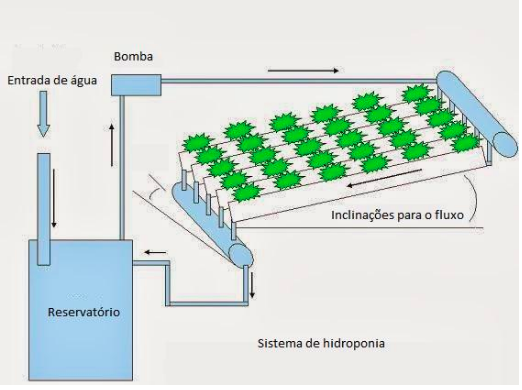
\includegraphics[width=13cm]{figuras/plantario.png}
	\caption{Plantário.}
	\label{plantario}
\end{figure}

De acordo com Silva et al. \cite{SILVA}, a vazão ideal no para uma estrutura hidropônica está entre 1,5 litro/minuto e 2,0 litros/minuto por canaleta de cultivo.

\section{Fundamentação alimentação}

O objetivo de uma fonte de alimentação é converter o fornecimento de tensão da rede elétrica (de 220V em corrente alternada (AC)) para uma outra tensão de corrente contínua (DC), que é geralmente drenada por aparelhos eletrônicos. Além disso, a fonte de alimentação filtra ruídos que possam ocorrer e estabilizam a corrente que vai ser fornecida \cite{SILVA}. 